% !TeX spellcheck = de_DE
% !TEX encoding = UTF-8
% !TEX TS-program = pdflatex
% !TEX root = ../tesi.tex

%**************************************************************
\chapter{Introduzione}
\label{cap:introduzione}
%**************************************************************
\section{Descrizione IQ Puzzler}
Lo scopo di IQ Puzzler è quello di riempire la griglia di gioco con tutte le varie forme a disposizione. Queste forme sono di varia dimensione, colore e struttura, e possono essere combinate in diversi modi per completare la griglia.\\
Il gioco comprende anche 100 configurazioni iniziali, dove alcune forme sono già posizionate all'interno della griglia e solo le rimanenti devono essere piazzate. All'aumentare delle forme rimanenti, aumenta notevolmete la complessità del gioco.\\ 
\begin{figure}[h]
	\centering
	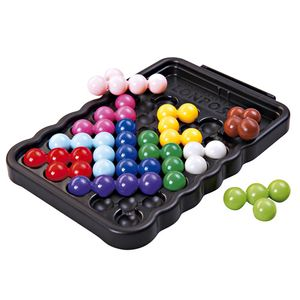
\includegraphics[scale=0.5]{immagini/iqpuzzler}
	\caption{Le forme di gioco di IQ Puzzler.}
	\label{fig:iqpuzzler}
\end{figure}

\newpage
\subsection{Forme di gioco}
Le forme totali sono 11, ognuna con una propria struttura diversa dalle altre, e sono formate da dei pallini collegati in modo da essere inseriti nelle celle della griglia.

\begin{figure}[h]
	
	\begin{minipage}{3.5cm}
		\centering
		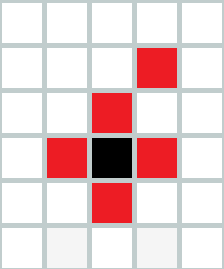
\includegraphics[scale=0.30]{immagini/p}
		\caption{}
		\label{p}
	\end{minipage}
	\ \hspace{2mm} \hspace{3mm} \
	\begin{minipage}{3.5cm}
		\centering
		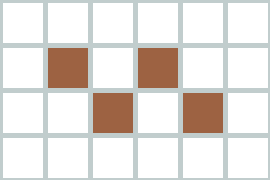
\includegraphics[scale=0.30]{immagini/z}
		\caption{}
		\label{z}
	\end{minipage}
	\ \hspace{2mm} \hspace{3mm} \
	\begin{minipage}{3.5cm}
		\centering
		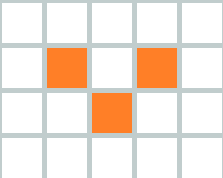
\includegraphics[scale=0.30]{immagini/smallv}
		\caption{}
		\label{smallv}
	\end{minipage}
\end{figure}

\begin{figure}[h]
	
	\begin{minipage}{3.5cm}
		\centering
		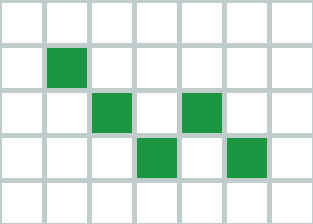
\includegraphics[scale=0.30]{immagini/bigz}
		\caption{}
		\label{bigz}
	\end{minipage}
	\ \hspace{2mm} \hspace{3mm} \
	\begin{minipage}{3.5cm}
		\centering
		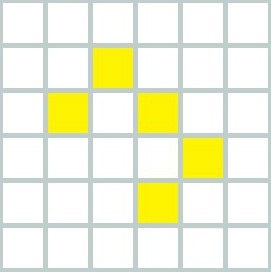
\includegraphics[scale=0.25]{immagini/yellow}
		\caption{}
		\label{c}
	\end{minipage}
	\ \hspace{2mm} \hspace{3mm} \
	\begin{minipage}{3.5cm}
		\centering
		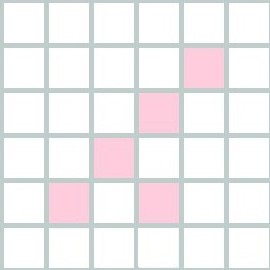
\includegraphics[scale=0.25]{immagini/Y}
		\caption{}
		\label{y}
	\end{minipage}
\end{figure}

\begin{figure}[h]
	
	\begin{minipage}{3.5cm}
		\centering
		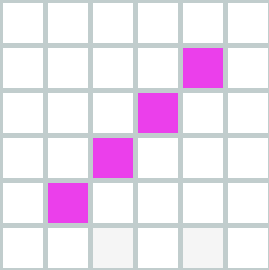
\includegraphics[scale=0.30]{immagini/i}
		\caption{}
		\label{i}
	\end{minipage}
	\ \hspace{2mm} \hspace{3mm} \
	\begin{minipage}{3.5cm}
		\centering
		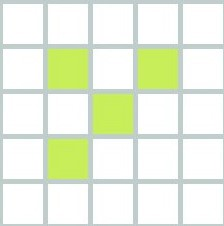
\includegraphics[scale=0.25]{immagini/T}
		\caption{}
		\label{t}
	\end{minipage}
	\ \hspace{2mm} \hspace{3mm} \
	\begin{minipage}{3.5cm}
		\centering
		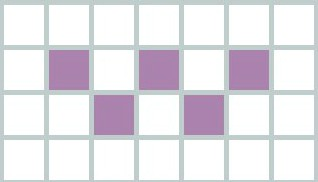
\includegraphics[scale=0.25]{immagini/w}
		\caption{}
		\label{w}
	\end{minipage}
\end{figure}

\begin{figure}[h]
	\centering
	\begin{minipage}{3.5cm}
		\centering
		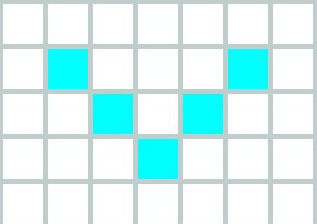
\includegraphics[scale=0.25]{immagini/v}
		\caption{}
		\label{v}
	\end{minipage}
	\ \hspace{2mm} \hspace{3mm} \
	\begin{minipage}{3.5cm}
		\centering
		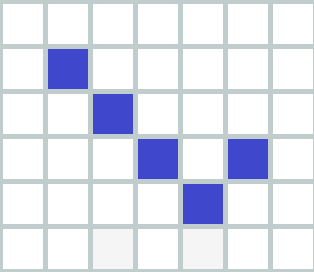
\includegraphics[scale=0.30]{immagini/L}
		\caption{}
		\label{l}
	\end{minipage}
\end{figure}

\newpage
\subsection{Griglia di gioco}
La griglia è formata da 11 righe con 4 o 5 celle, dove ogni cella è collegata solo con quelle nelle sue 2 diagonali. In totale la griglia è formata da 50 celle.

\begin{figure}[h]
	\centering
	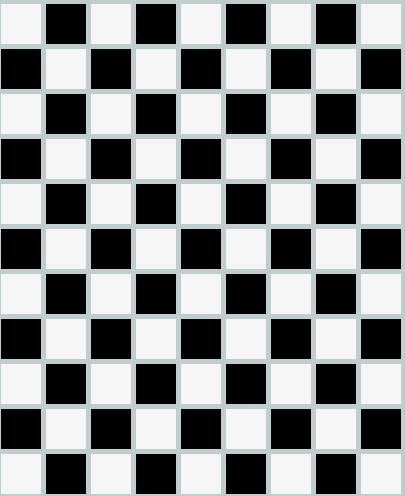
\includegraphics[scale=0.3]{immagini/griglia}
	\caption{La griglia di gioco di IQ Puzzler. Le forme possono essere piazzate utilizzando solo le celle bianche.}
	\label{fig:griglia}
\end{figure}


\newpage
\section{Scopo del progetto}
Lo scopo del nostro progetto è stato quello di ricreare questo gioco ed implementare alcuni dei metodi risolutivi visti durante il corso di Intelligenza Artificiale per risolverlo. \\
In un secondo momento abbiamo confrontato le performance dei vari algoritmi in modo da valutare la loro efficienza rispetto a questo problema.

\section{PEAS}

\subsection{Performance measure}
\label{performance}
La misura di performance è il tempo impiegato da un algoritmo per risolvere il problema a partire da una delle configurazioni iniziali. Oltre al tempo, abbiamo anche considerato il numero di azioni necessarie per raggiungere una soluzione, in maniera tale da poter fare osservazioni più precise su alcuni tipi di solver.\\
Tuttavia, la misura di performance più importante rimane la prima.

\subsection{Environment}
Il gioco analizzato presenta un ambiente totalmente osservabile, deterministico, sequenziale, statico, discreto e single-agent.  L'ambiente è completamente determinato dallo stato corrente e dall'agente che può effettuare una sola mossa alla volta.
L'azione dell'agente determina le azioni future dato che il possibile cammino
si riduce ad ogni passo.

\subsection{Actuators}
Il programma rappresenta l'esecuzione di un'azione attraverso la colorazione delle celle assegnate ad una determinata forma (passo di computazione).

\subsection{Sensors}
Ad ogni passo di computazione l'input della funzione agente è rappresentato dalla griglia e dalle forme rimanenti da inserire.

\section{Formalizzazione del problema}
\begin{itemize}
	\item \textbf{Stato inziale}: configurazione iniziale (possibilmente anche vuota) della griglia e relative forme mancanti da inserire;
	\item \textbf{Azioni possibili}: tutti i possibili modi di inserire una forma non ancora presente nella griglia;
	\item \textbf{Transition model}: colorazione, a seconda del colore della forma, della posizione scelta nella griglia;
	\item \textbf{Test obiettivo}: controllare se tutte le forme sono state inserite nella griglia, in modo da riempirla completamente;
	\item \textbf{Path cost}: tempo necessario per raggiungere la soluzione.
					
\end{itemize}

\section{Strumenti utilizzati}
Il programma è stato completamente sviluppato in Python 3.6 con l'utilizzo della libreria \textit{pygame} per quanto rigurda la parte grafica, e la libreria \textit{python-constraint} per la risoluzione del problema formulato come CSP. \\
La libreria \textit{python-constraint} è stata inoltre modificata e inclusa nella cartella \texttt{pythonConstraint/} per due motivi:
\begin{itemize}
	\item apportare delle migliorie agli algoritmi presenti, che verranno esposte successivamente nel documento;
	\item permettere di visualizzare ogni assegnamento parziale durante l'esecuzione dell'algoritmo.
\end{itemize}  

\section{Utilizzo del programma}
Per poter utilizzare il programma è necessario:
\begin{itemize}
	\item aver installato nel computer Python 3;
	\item spostarsi con il terminale alla cartella radice (\texttt{IQPuzzlerSoler/}) contenente il programma;
	\item eseguire uno di questi due comandi:
	\begin{itemize}
		\item \begin{verbatim}
		python main.py
		\end{verbatim}inizia l'esecuzione del programma, guidando l'utente nella scelta della difficoltà del problema e in che modo risolverlo. Le possibili difficoltà sono 5 (da 0 a 4) e di complessità crescente. I metodi di risoluzione sono quattro, ognuno dei quali permette di scegliere se utilizzare tale metodo con le migliorie ideate e implementate da noi (descritte in \ref{migliorie}) o meno; 
		\item \begin{verbatim}
		sh Test/scriptTest.sh
		\end{verbatim}esegue automaticamente una serie di esempi di problemi con vari metodi di risoluzione, tracciando i risultati ottenuti nel file \texttt{Test/testResult.txt}. 
	\end{itemize}
\end{itemize}
\begin{figure}[h]
	\centering
	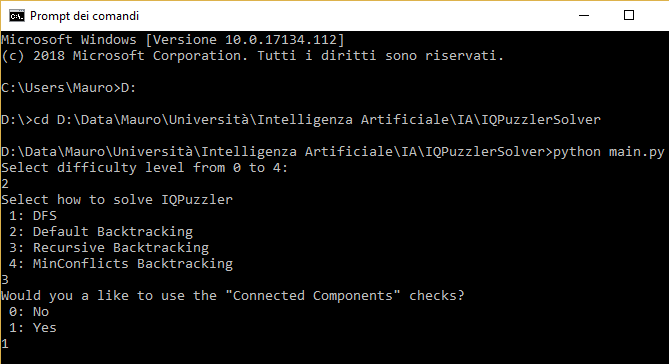
\includegraphics[scale=0.65]{immagini/exe}
	\caption{Esempio di esecuzione del programma}
	\label{fig:exe}
\end{figure}


